% --- Ha \& Schmidhuber (2018): V--M--C architecture ---
\begin{frame}{World Model Overview}
    \centering
    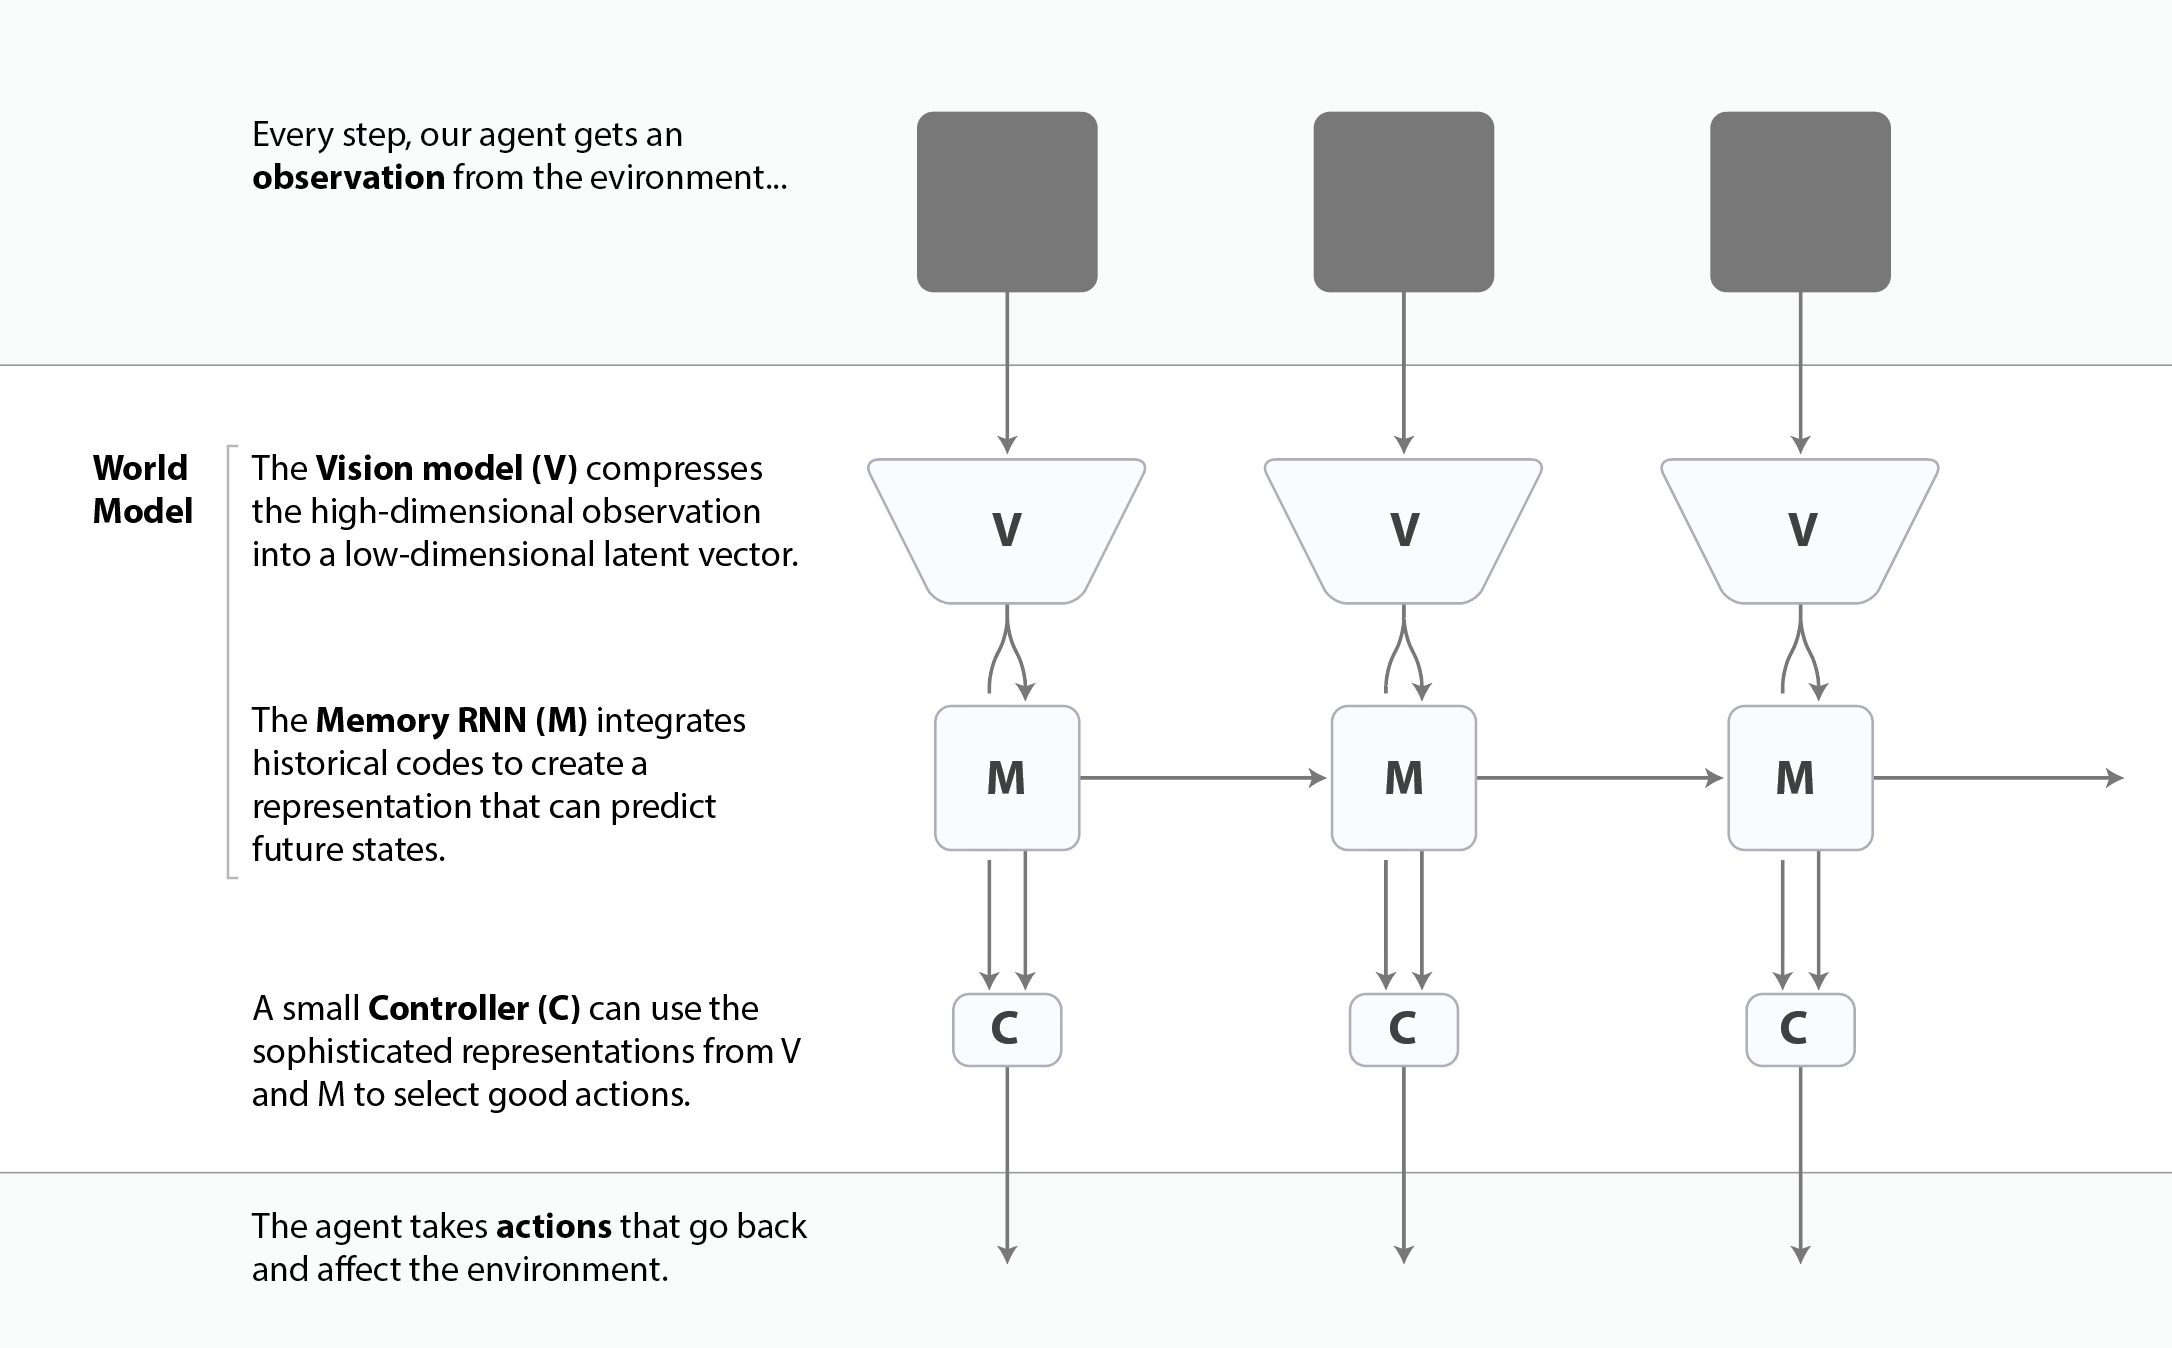
\includegraphics[width=0.95\linewidth,height=0.88\textheight,keepaspectratio]{images/world-models/worldmodels_githubio_rollout_schematic.png}\\[0.15em]
    {\scriptsize World model overview.\\
    \textit{Source: Ha \& Schmidhuber, 2018}}
\end{frame}

\begin{frame}{Vision module: variational autoencoder (V)}
  \begin{columns}[T,onlytextwidth]
    \column{0.44\textwidth}
    \begin{itemize}\itemsep0.26em
      \item[\textcolor{red}{$\blacktriangleright$}] \textbf{Goal:} learn an abstract, compressed representation of each observed input frame.
      \item[\textcolor{red}{$\blacktriangleright$}] \textbf{VAE:} first stage of a two-stage sequence model; similar in spirit to modern tokenizers, but trained with the classic VAE objective (see the background slide).
    \end{itemize}
    \column{0.54\textwidth}
    \centering
    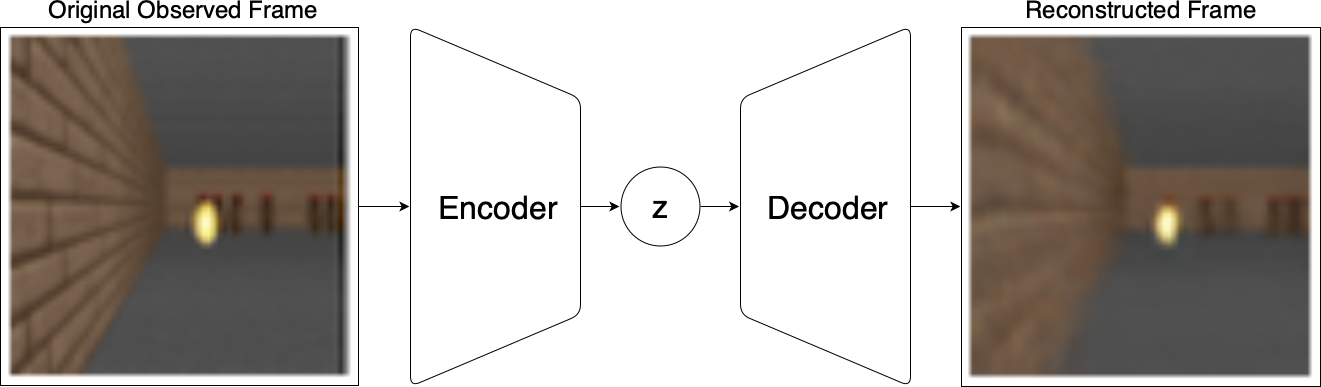
\includegraphics[width=0.95\linewidth,height=0.88\textheight,keepaspectratio]{images/world-models/worldmodels_githubio_vae.png}\\[0.15em]
    {\scriptsize VAE diagram.\\
    \textit{Source: Ha \& Schmidhuber, 2018}}
  \end{columns}
\end{frame}

\begin{frame}{Memory module: MDN-RNN (M)}
  \begin{columns}[T,onlytextwidth]
    \column{0.42\textwidth}
    \begin{itemize}\itemsep0.26em
      \item[\textcolor{red}{$\blacktriangleright$}] Model $p(z_{t+1} \mid z_t, a_t, h_t)$ where $z_t$ is the latent state at time $t$, $a_t$ is the action at time $t$, and $h_t$ is the hidden state at time $t$.
      \item[\textcolor{red}{$\blacktriangleright$}] \textbf{MDN-RNN:} an RNN (LSTM, from the RNN lecture) whose output parameterizes a \textbf{mixture of Gaussians} over the next latent $z_{t+1}$; a mixture can represent several plausible futures at once.
      \item[\textcolor{red}{$\blacktriangleright$}] A temperature parameter $\tau$ scales the sampling uncertainty; it becomes important when training inside the dream.
    \end{itemize}
    \column{0.56\textwidth}
    \centering
    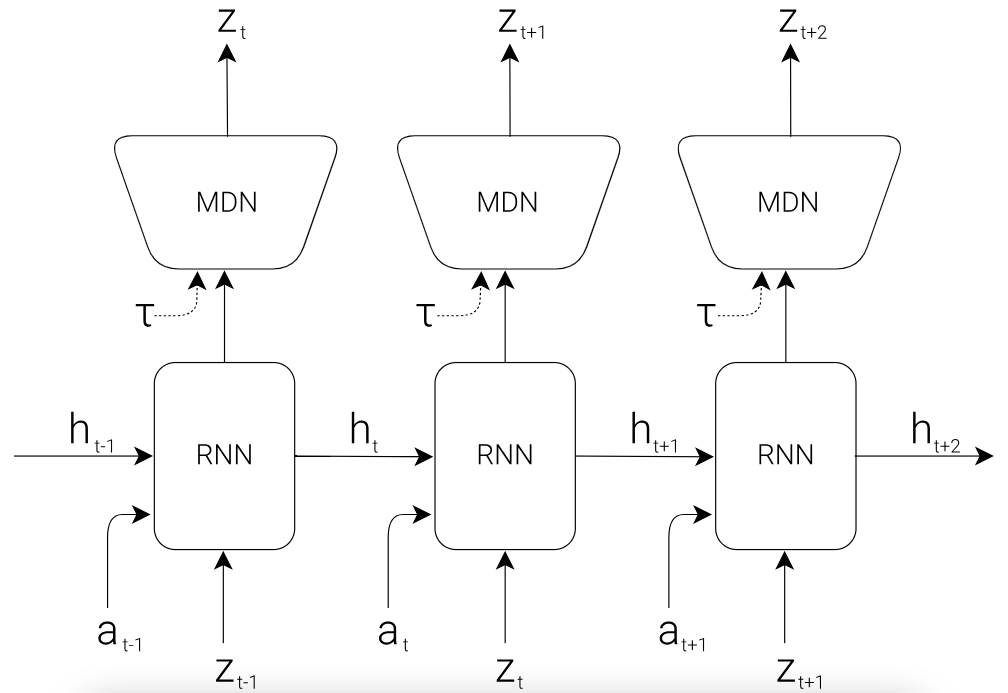
\includegraphics[width=0.95\linewidth,height=0.76\textheight,keepaspectratio]{images/world-models/mdn_rnn_new.png}\\[0.15em]
    {\scriptsize MDN-RNN architecture.\\
    \textit{Source: Ha \& Schmidhuber, 2018}}
  \end{columns}
\end{frame}


\begin{frame}{Controller module: decision-making (C)}
    \begin{itemize}\itemsep0.26em
      \item[\textcolor{red}{$\blacktriangleright$}] The \textbf{Controller (C)} selects actions to maximize expected cumulative reward during agent rollout.
      \item[\textcolor{red}{$\blacktriangleright$}] Designed to be as simple and small as possible; trained \textbf{separately} from the Vision (V) and Memory (M) modules.
      \item[\textcolor{red}{$\blacktriangleright$}] Most agent complexity is thus concentrated in the world model (V and M).
      \item[\textcolor{red}{$\blacktriangleright$}] C is a \textbf{single-layer linear} model that maps the latent vector $z_t$ and RNN hidden state $h_t$ directly to the action $a_t$ at each time step:
    \end{itemize}
    {\small
    \[
      a_t = W_c [z_t; h_t] + b_c
    \]
    }
    \begin{itemize}\itemsep0.15em
      \item[\textcolor{red}{$\blacktriangleright$}] $W_c$ and $b_c$ are the weight matrix and bias; $[z_t; h_t]$ is the concatenated latent and memory state, and $a_t$ the resulting action.
      \item[\textcolor{red}{$\blacktriangleright$}] Because C has only a few hundred parameters, it is trained with \textbf{CMA-ES}, an evolution strategy that searches weight space directly; no gradients through the agent loop are needed.
    \end{itemize}
\end{frame}

\begin{frame}{World model: Putting Everything Together}
  \centering
  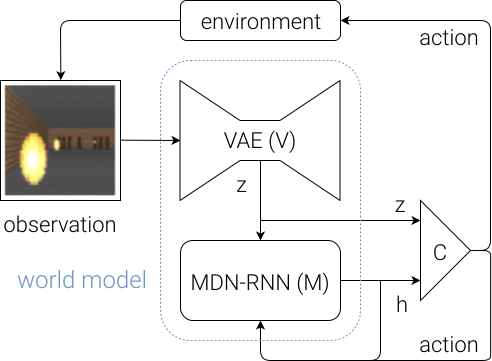
\includegraphics[width=\linewidth,height=0.85\textheight,keepaspectratio]{images/world-models/world_model_schematic_downloads.png}\\[0.28em]
  {\scriptsize Agent-environment flow (observation $\rightarrow$ $z_t$, RNN state $h_t$, action $a_t$, next step).\\
  \textit{Source: Ha \& Schmidhuber, 2018}}
\end{frame}
% --- Training inside the dream ---
\begin{frame}{Training Inside the Dream}
  \begin{itemize}\itemsep0.3em
    \item The memory model M can generate its own environment: replace real observations with imagined latents and train the controller \textbf{entirely inside the hallucinated rollout}.
    \item In the VizDoom experiment, a policy trained purely in the dream \textbf{transfers back to the real game} (as reported in the paper).
    \item The failure mode: the controller learns to \textbf{exploit model errors}, steering into states the model predicts wrongly (for example, imagined worlds where enemies never fire).
    \item Countermeasure: raise the temperature $\tau$ so the dream is noisier and harder to exploit; the resulting policy is more robust in the real environment.
    \item This exploit-the-model problem returns in Dreamer, handled there with KL constraints on the latent dynamics.
  \end{itemize}
\end{frame}

\begin{frame}{Takeaways}
  \begin{itemize}
    \item \textbf{Separation of concerns:} perception (VAE), dynamics (RNN), decision (controller). Easy to prototype, but the modules do \textbf{not} share gradients end-to-end through the full agent loop at scale.
    \item \textbf{Stochastic latents} matter: the world is multi-modal; Gaussian or MDN heads encode ``many possible futures''.
    \item Next step (PlaNet, Dreamer): unify training with \textbf{RSSM}-style latent dynamics and \textbf{model-based RL} losses.
  \end{itemize}
\end{frame}
